\chapter{Basic Knowledge}

\section{Roundabouts}
Kreisverkehre erfreuen sich in Deutschland an steigender belibetheit. \todo{referenz} Wie in \cref{conflict_roundabout} zu sehen  haben sie eine kleinere Anzhahl an Konflikktpunkten (8)
im gegensatz zu kreuzungen (32) und  tragen daher stark zur sicherheit im Straßenverkehr bei, was die Unfallrate Reduziert

\begin{figure}[!ht]
  %\addcontentsline{lof}{figure}{LaTeX--Strukturelemente}
%\begin{center}
\caption{Roundabout Conflict Points \cite{man06}}
 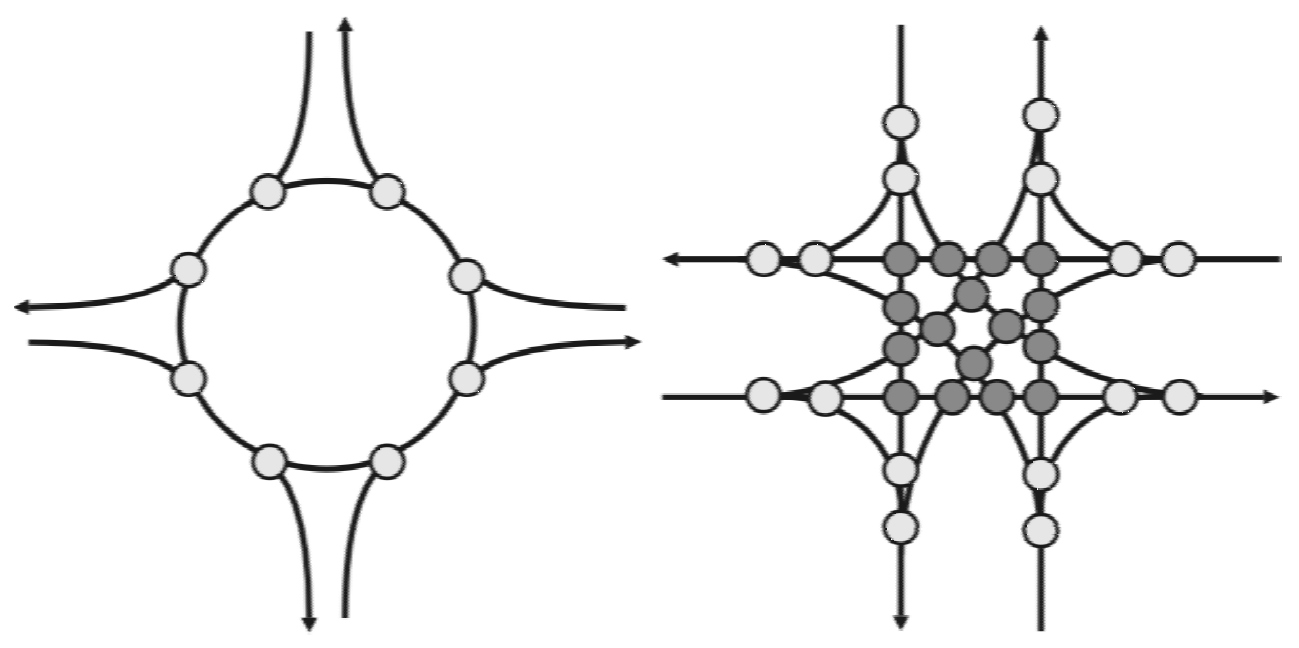
\includegraphics[width=\textwidth]{bilder/conflict.png}
\label{conflict_roundabout}
%\end{center}
\end{figure}

So lag im Jahre 2009 bei einer Untersuchung \cite{Bondzio2012}, von 54426 Unfällen im Innenstadtbereich, die Anzahl der Unfälle in Kreisverkehren bei nur 1150 (2.1\%) [\cref{unfall_roundabout}].
Weiterhin erlauben es Kreisverkehre auch Knotenpunkte mit mehr als 4 Straßen zu konstuieren, was ihnen einen weiteren Vorteil verschafft.
Leider gibt es diesbezüglich im Rahmen des autonomen fahrens nur wenige Veröffentlichungen.
%\definecolor{myblue}{HTML}{92dcec}

\begin{figure}[!ht]
  %\addcontentsline{lof}{figure}{LaTeX--Strukturelemente}
%\begin{center}
\caption{Accidents in City Limits \cite{Bondzio2012}}
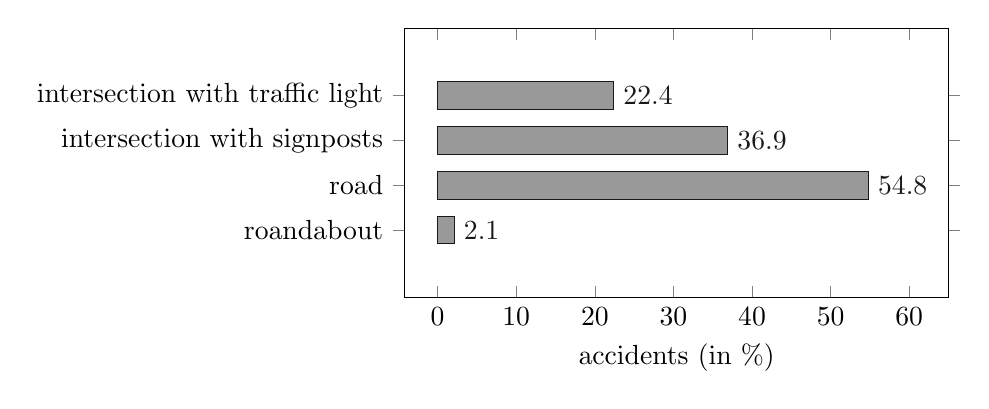
\begin{tikzpicture}
  \begin{axis}[
    xbar,xmax=65, width=0.7\textwidth, height=5cm, enlarge y limits=0.5, xlabel={accidents (in \%)},
    symbolic y coords={roandabout,road,intersection with signposts,intersection with traffic light}, ytick=data,
    nodes near coords, nodes near coords align={horizontal}, ]
    \addplot[gray!20!black,fill=gray!80!white] coordinates {(2.1,roandabout) (54.8,road) (36.9,intersection with signposts) (22.4 ,intersection with traffic light)};
  \end{axis}
\end{tikzpicture}
\label{unfall_roundabout}
%\end{center}
\end{figure}

Auch wenn Kreisverkehre für den Menschlichen Fahrer scheinbar eine Erleichterung darstellen, ist es nötig die Herausforderungen in hinblick aufbaudas Autonome Fahren zu Untersuchen.
Dazu gibt es im Folgenden eine übersicht der Rechtlichen aspekte in Deustschland.


\subsection{Roundabouts in Law}
% In Deutschland gibt es kein Gesetzt was den genauen Konstuktion von Kreisverkehren vorschreibt.
% Stattdessen werden die Elemente der Landstraßen und Stadtstraßen in Richtlinien für die Anlage von Landstraßen (RAL) bzw.
% den Richtlinien für die Anlage von Stadtstraßen (RASt) behandelt. Diese Richtlinien sind auch für die
% Wahl einer zweckmäßigen Knotenpunktart bei der Verknüpfung von Straßen maßgebend. Für diese Abreit sind die 
% Richtlinien für die Anlage von Stadtstraßen (RASt) relevant. Die dort behandelten Abwägungsüberlegungen orientieren sich an verkehrlichen Größen, umfeldbezogenen Merkmalen,
% wirtschaftlichen Kriterien und raumordnerischen oder städtebaulichen Vorgaben. Die Richtlinien regeln auch grundlegend die entwurfstechnische und betriebliche Ausbildung von Kreisverkehren.
%
In Germany, there is no law stipulating the exact construction of roundabouts.
Instead, the elements of the rural roads and city streets are dealt with in ``Directives for the Design of rural roads'' \cite{ral13}
and the ``Directives for the Design of Urban Roads''  \cite{rast06}. These guidelines are also relevant to the choice of a convenient junction type when linking roads.
The considerations discussed there are based on traffic variables, area-related characteristics, economic criteria and spatial planning or urban planning requirements. 
The guidelines also regulate the basic design and operational formation of roundabouts.
The  Directives for the Design of Urban Roads \cite{rast06} are relevant for this dispute. Since the access the RASt ist limited, most of the information is coming from
\cite{man06} whereupon RASt is based on.
\subsection{Elements of a Roundabout}

\begin{figure}[!ht]
%%\begin{center}
\caption{Definition of individual design elements and dimensions of a roundabout \cite{man06}}
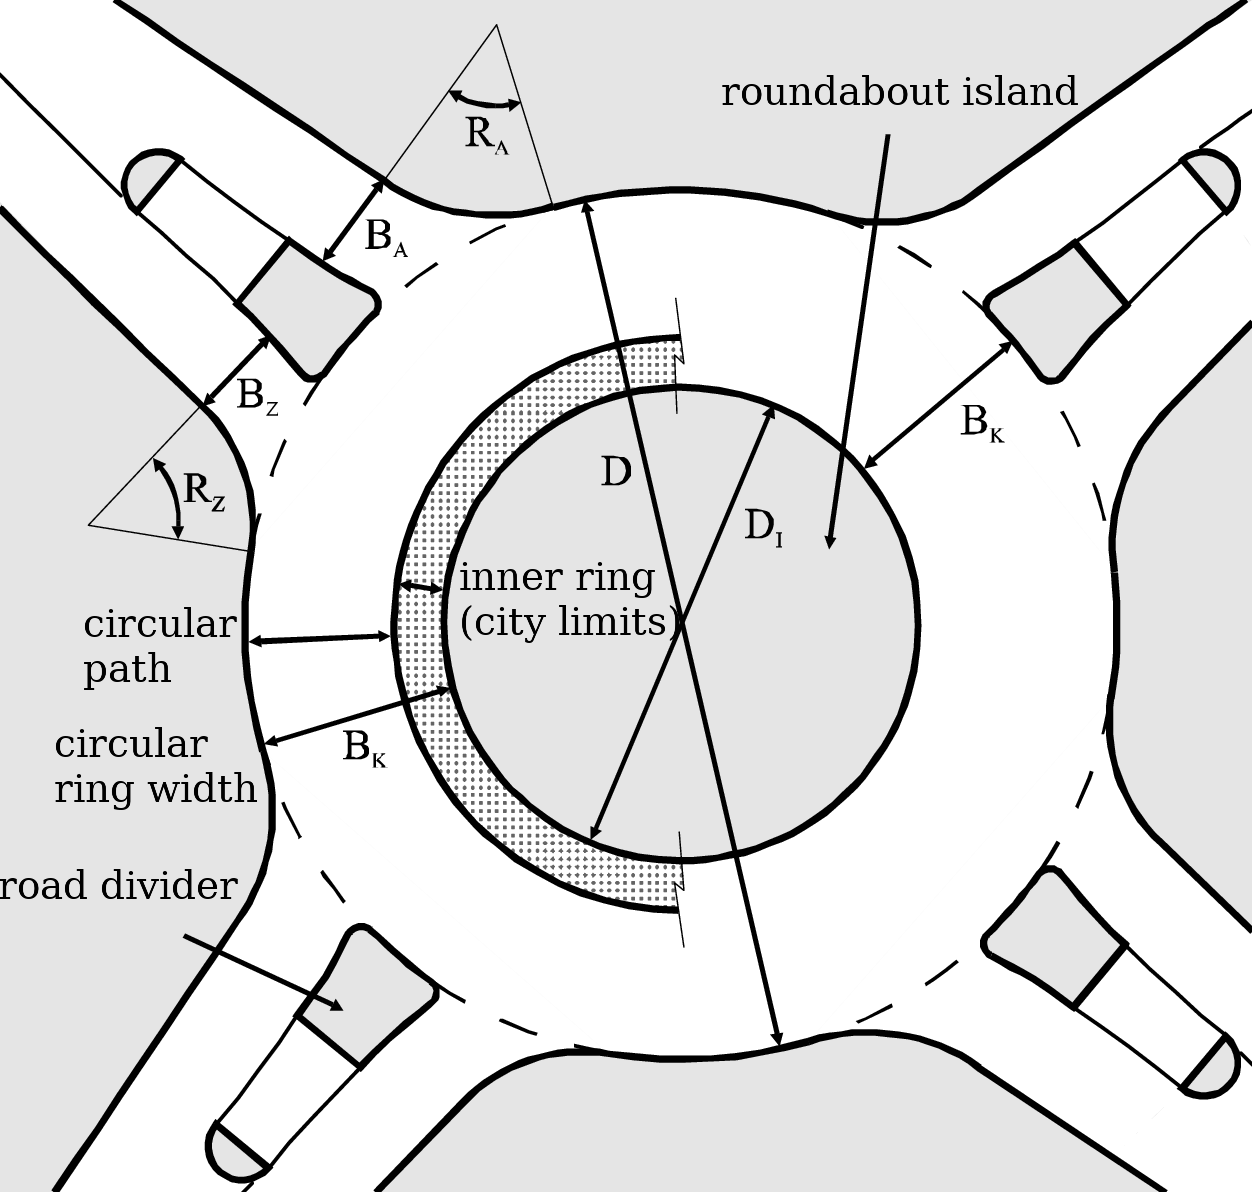
\includegraphics[width=0.7\textwidth]{bilder/kreisverkehr.png} %70% der Textbreite
\label{roundabout_parts}
%%\end{center}
\end{figure}


\begin{defi}[roundabout island]
The roundabout island is the constructional area in the middle of the roundabout, which is surrounded by vehicles.
For miniature roundabouts, the roundabout island is crossable. \cite{man06}
\end{defi}

\begin{defi}[circular path]
%Die Kreisfahrbahn ist die Fahrbahn, die zum Umfahren der Kreisinsel
%dient. Ein ggf. vorhandener Innenring ist verkehrsrechtlich nicht Be-
%standteil der Kreisfahrbahn (VwV-StVO zu §9a V., Rn. 5).

%%TODO
The circular path is the road that serves to drive the roundabout island. An inner ring, if present, is not part of the circular path (VwV-StVO zu §9a V., Rn. 5). \cite{man06}
\end{defi}

\begin{defi}[circular ring with ($B_K$)]
% Die bauliche Breite umfasst die Kreisfahrbahn und einen ggf. gepflasterten
% Innenring. Sie ist abhängig vom Außendurchmesser und der angestrebten
% Verkehrsführung (ein- oder zweistreifig). Die Randstreifenbreite orientiert
% sich an der maßgebenden durchgehenden Fahrbahn.
The structural width includes the circular track and a paved inner ring, if any. It is dependent on the outer diameter and the desired traffic routeing (one or two lanes). 
The edge strip width is oriented on the relevant continuous roadway. \cite{man06}
\end{defi}

\begin{defi}[outer diameter ($D$)]
The outer diameter is measured at the outer edge of the circular ring. It is the essential measure for describing the size of the roundabout. \cite{man06}
\end{defi}

\begin{defi}[inner diameter ($D_I$)]
The inner diameter is the diameter of the roundabout island. \cite{man06}
\end{defi}

\begin{defi}[road divider]
% Der Fahrbahnteiler ist die baulich ausgeführte Insel zwischen Kreisausfahrt
% und -zufahrt einer angeschlossenen Straße. Er dient der Trennung der
% Kreisaus- und -zufahrten, der Führung des Verkehrs sowie den Fußgängern
% und Radfahrern als Überquerungshilfe.
%
The road divider is the structurally designed island between the circular exit
and circular driveway. It serves to separate the circular exit and circular driveway, the management of the traffic, as well as the pedestrians and cyclists as cross-bordering aid. \cite{man06}
\end{defi}

\begin{defi}[lane width of the circular driveway ($B_Z$) and circular exit ($B_A$)]
% Die Breite der Kreiszufahrt und Ausfahrt wird am Beginn der Eckausrundung gemessen.
The width of the circular driveway and exit is measured at the beginning of the corner. \cite{man06}
\end{defi}

\begin{defi}[Corner rounding radius ($R_Z$ and $R_A$) ]
% Dies ist der Radius der Ausrundung am rechten Fahrbahnrand zwischen 
% der Kreiszufahrt und der Kreisfahrbahn. Bei einem Korbbogen mit einer
% Radienfolge aus drei unterschiedlichen Radien ist RZ der Radius R2 des
% mittleren Bogens. Bei der Ausbildung des Fahrbahnrandes als Schleppkurve ist RZ der kleinste Radius des Fahrbahnrandes.
% 
This is the radius of the rounding at the right edge of the road between the circular driveway and the circular path.
For a elliptical arch with a radius sequence of three different radii, $R_Z$ is the radius $R_2$ of the central arc.
When the road edge is formed as a tractrix, $R_Z$ is the smallest radius of the road edge. \cite{man06}
\end{defi}

\subsection{Types of Roundabouts}
\label{types_of_roundabouts}
There are several types of roundabouts, which are differentiated by the different application criteria and the partly different design principles according to the situation inside and outside built areas.
Furthermore, a division is made as a function of its size. \cite{man06}


\subsubsection{Mini Roundabout}

\begin{figure}[!ht]
%\begin{center}
\caption{Mini Roundabout \cite{man06}}
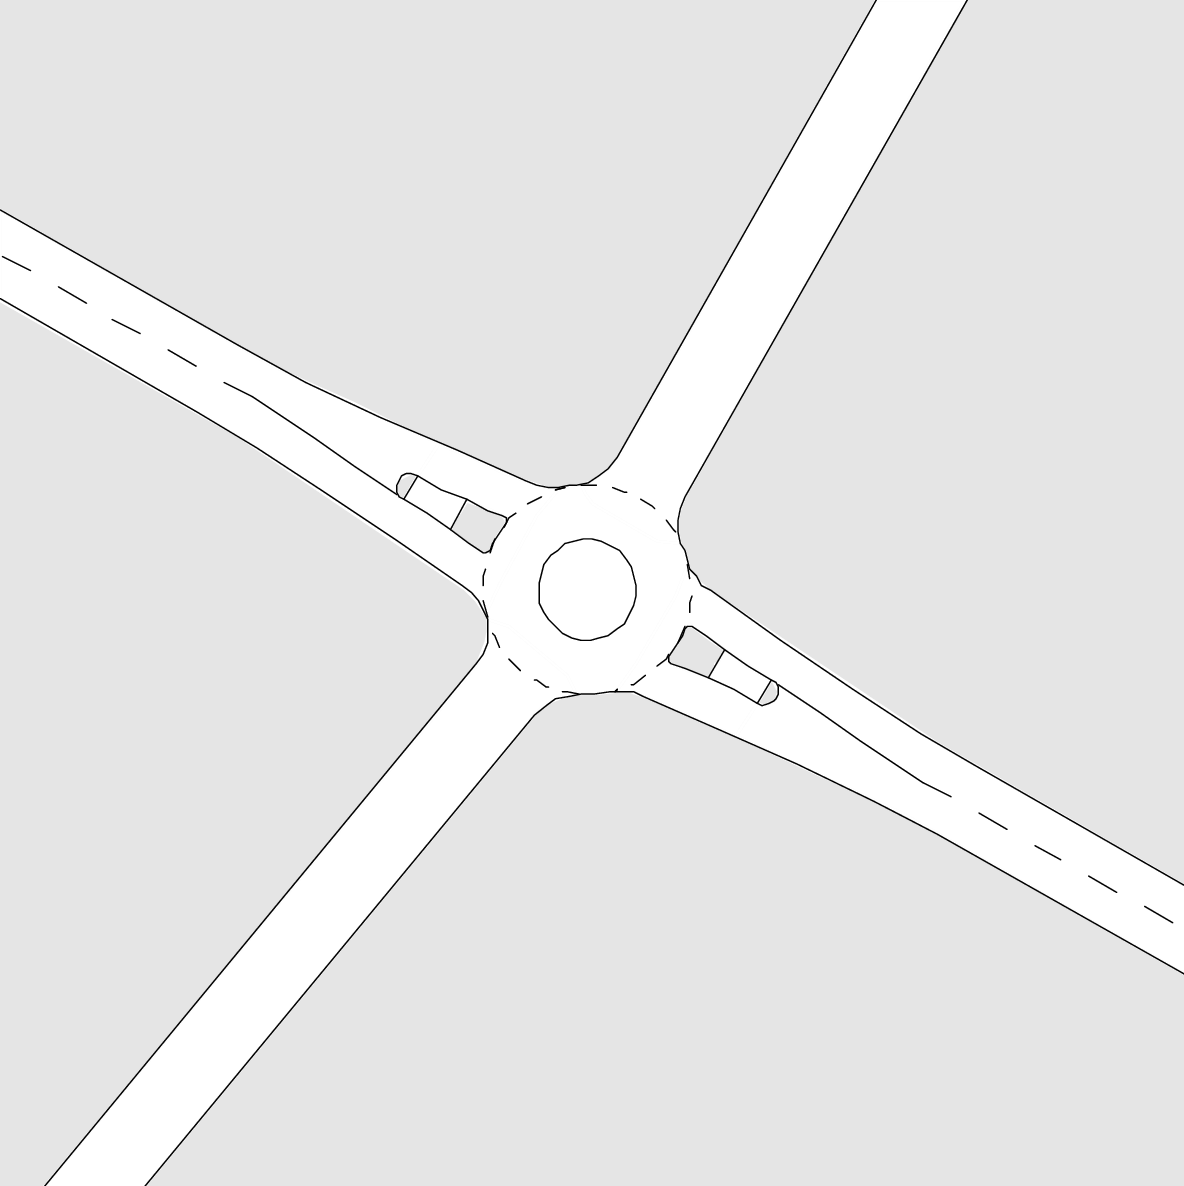
\includegraphics[width=0.5\textwidth]{bilder/mini_roundabout.png} %70% der Textbreite
\label{roundabout_mini}
%\end{center}
\end{figure}

Within built-up areas, smaller outer diameters are possible under certain conditions.
These roundabouts are called mini roundabout. The roundabout island must then be capable of being passed over.
The outer diameter should be at least 13 m, so that the circular island does not become too small.
Larger outer diameters make driving easier. Outer diameters of more than 22m, however, do not offer any transport advantages.
From an outside diameter of about 22 m, therefore, the installation of a small roundabout with 26 m is generally more convenient.
Bypasses are generally not required in the areas where mini roundabout can be used.


\subsubsection{Small Roundabout}

\begin{figure}[!ht]
%\begin{center}
\caption{Small Roundabout \cite{man06}}
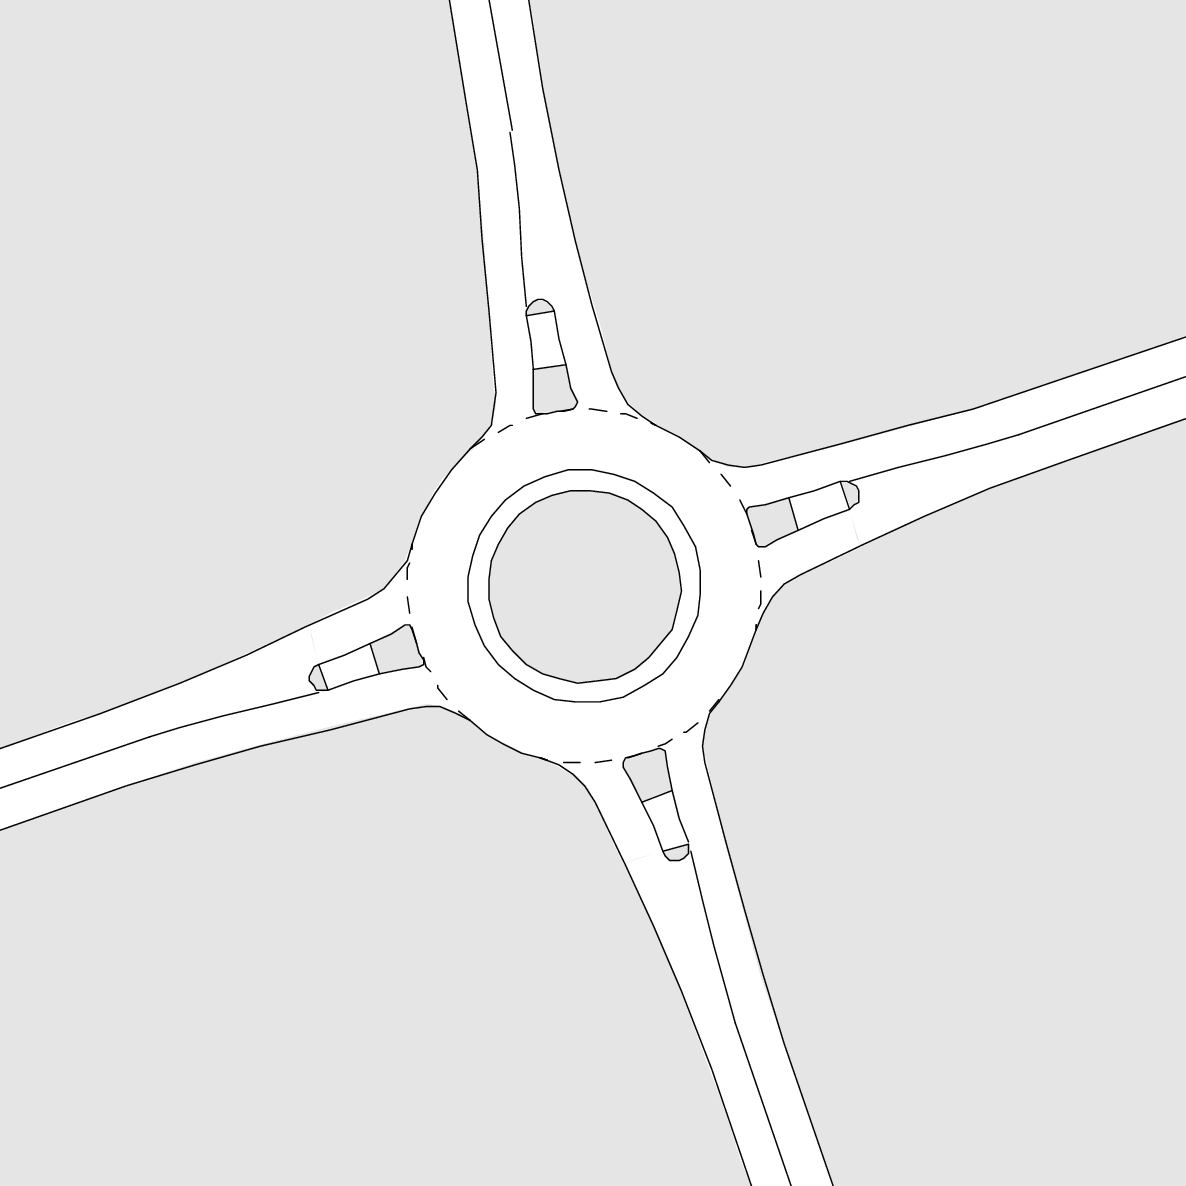
\includegraphics[width=0.5\textwidth]{bilder/small_roundabout.png} %70% der Textbreite
\label{roundabout_small}
%\end{center}
\end{figure}

The small roundabout has a single lane circular path and single lane circular driveways and exits. The roundabout island is not passable.
The outer diameter must be at least 26 m. Bypasses can be set up for driving geometric reasons or to increase performance.


\subsubsection{Two-lane Passable Roundabout}

\begin{figure}[!ht]
%\begin{center}
\caption{Two-lane Passable Roundabout \cite{man06}}
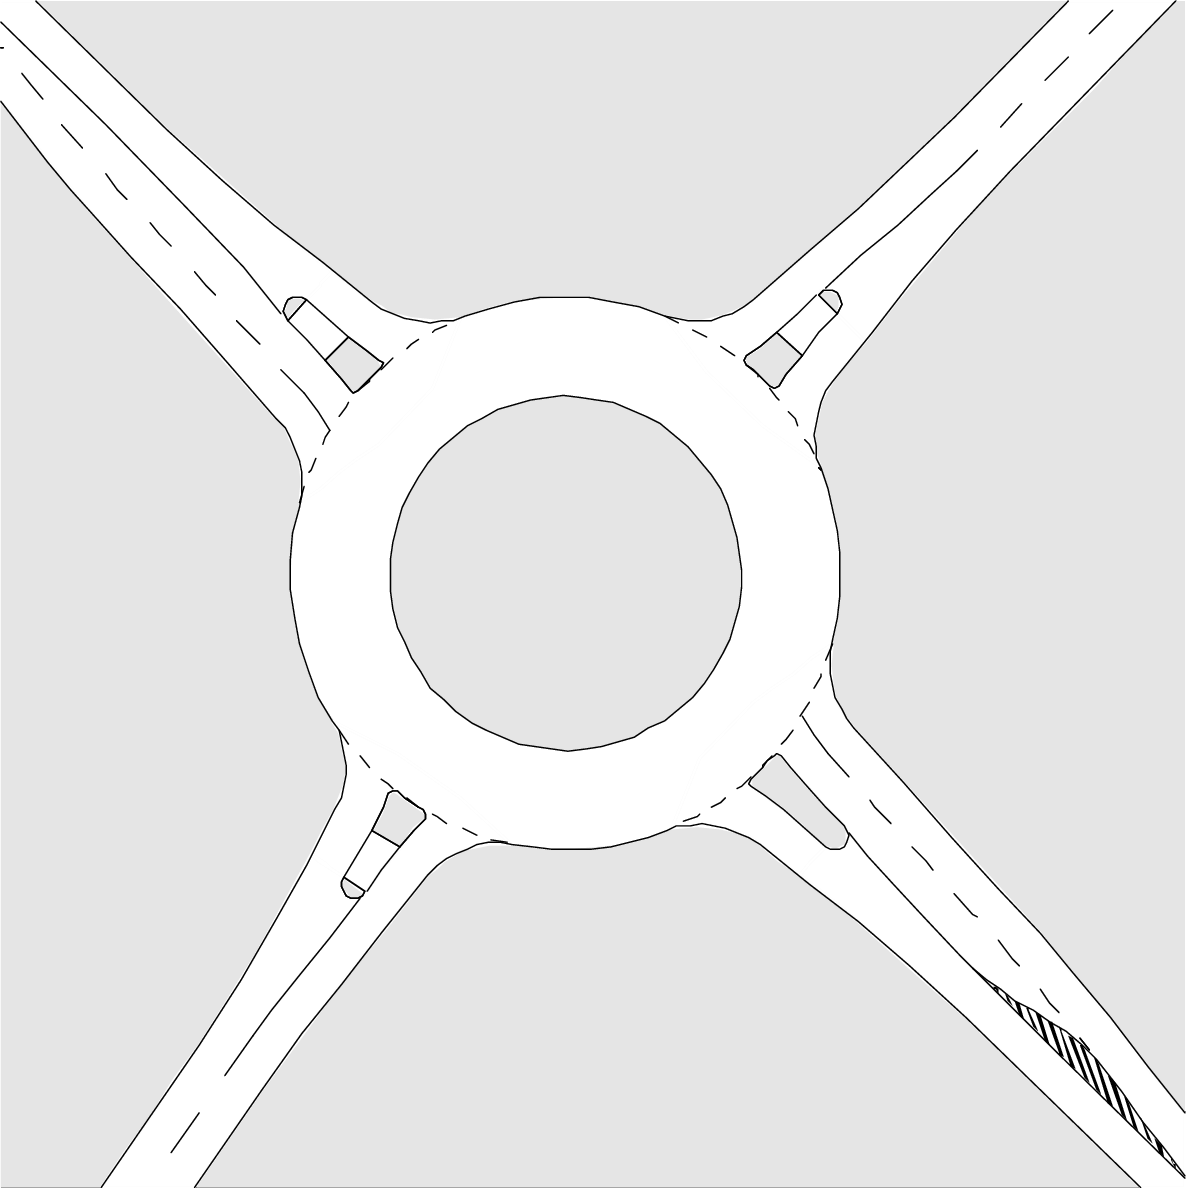
\includegraphics[width=0.5\textwidth]{bilder/twolaned_roundabout.png} %70% der Textbreite
\label{roundabout_twolaned}
%\end{center}
\end{figure}

% Reicht die Kapazität des Kleinen Kreisverkehrs nicht aus und kann diese nicht durch die Anlage von Bypässen sicher gestellt werden,
% kann die Kreisfahrbahn eines Kleinen Kreisverkehrs zweistreifig befahrbar ausgebildet werden.
% An einem solchen Kreisverkehr ist die Kreisfahrbahn so breit, dass Pkw im Kreis nebeneinander fahren können.
% Wird eine weitere Erhöhung der Kapazität erforderlich, können einzelne Kreiszufahrten ebenfalls zweistreifig ausgeführt werden,
% wenn Fußgänger und Radfahrer regelmäßig nicht zu berücksichtigen sind. Kreisausfahrten werden aus Sicherheitsgründen immer einstreifig ausgeführt.
% Aus geometrischen Gründen muss der Außendurchmesser bei zweistreifiger Befahrbarkeit mindestens 40 m betragen.
%
If the capacity of the small roundabout is not sufficient and can not be ensured by the installation of bypasses,
the circular path of a small roundabout can be designed to be two-lane driveable.
At such a roundabout, the circular path is so wide that cars can travel side by side in a circle.
If a further increase in the capacity is required, individual circular driveway can also be carried out in two lanes, if pedestrians and cyclists are not to be considered regularly.
For safety reasons, circular exits are always carried out in single lanes.
For geometrical reasons, the outer diameter must be at least 40 m for two-laned accessibility.


\subsubsection{Large Roundabout}


\begin{figure}[!ht]
%\begin{center}
\caption{Large Roundabout \cite{man06}}
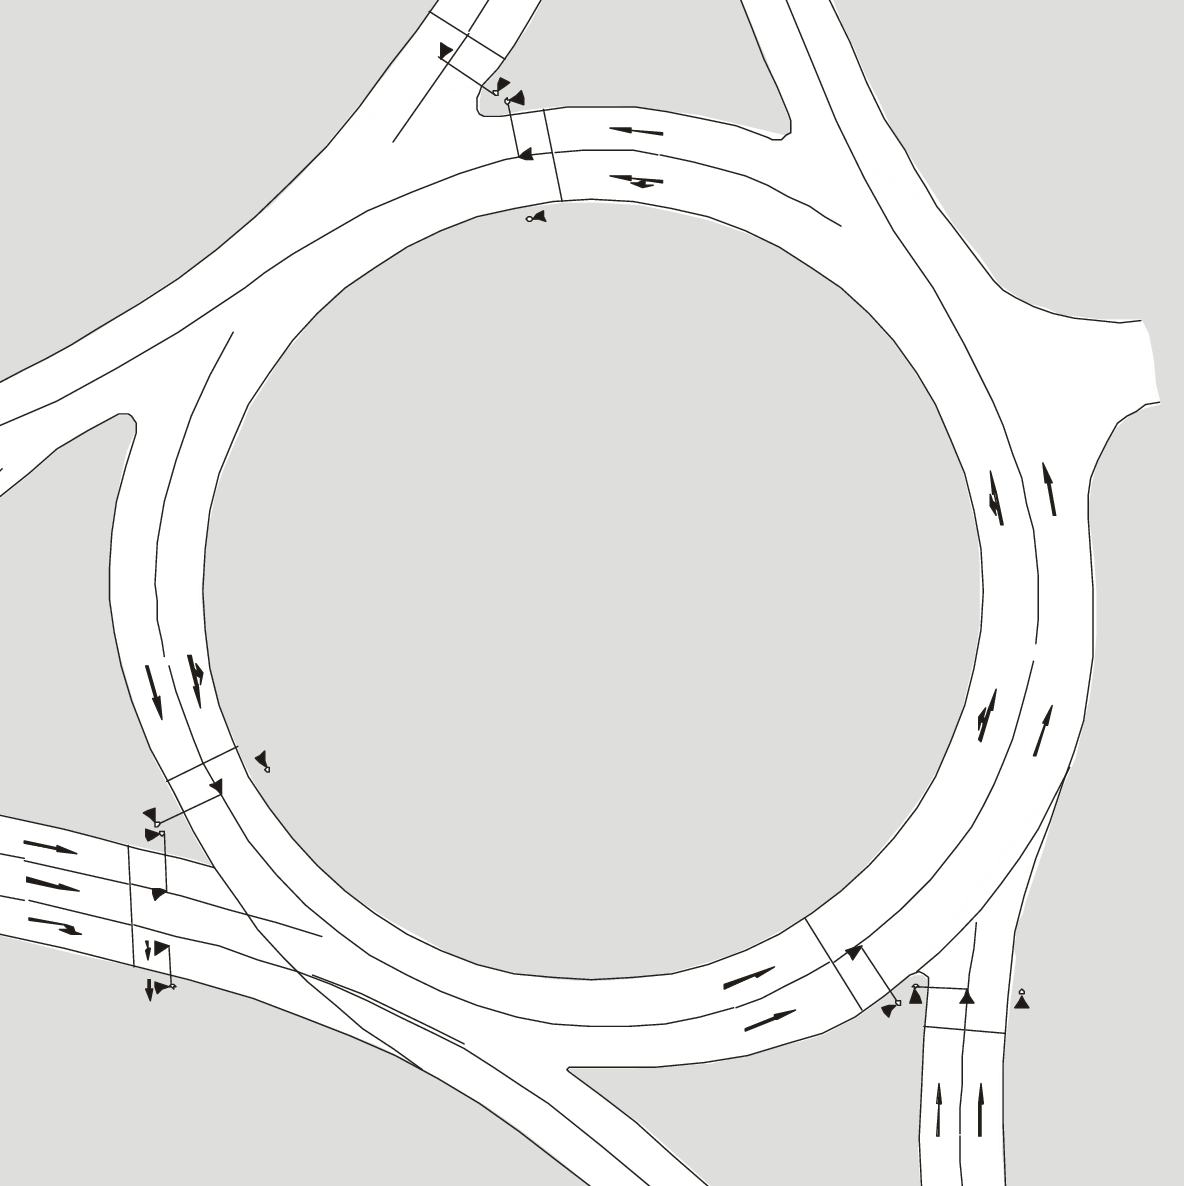
\includegraphics[width=0.5\textwidth]{bilder/large_roundabout.png} %70% der Textbreite
\label{roundabout_large}
%\end{center}
\end{figure}

%Große Kreisverkehre mit zwei oder mehreren durch Markierungen gekennzeichnete Fahrstreifen auf der Kreisfahrbahn sollen bei enger
%Abstimmung zwischen Knotenpunktentwurf und Verkehrssteuerung nur mit Lichtsignalanlage betrieben wer den.
Large Roundabouts with two or more lanes marked by markers on the circular path should be operated with a light signaling system only,
if the nodal point design and traffic control are closely coordinated.


\section{\acl{RANSAC}}

Der \ac{RANSAC} \cite{Fischler1981} ist ein Algorithmus zur Schätzung eines Modells innerhalb einer Reihe von Messwerten mit Ausreißern und groben Fehlern. Wegen seiner Robustheit wird er vor allem bei der Auswertung automatischer Messungen vornehmlich im Bereich der Bildverarbeitung. 
Hier unterstützt \ac{RANSAC} durch Berechnung einer um Ausreißer bereinigten Datenmenge, des sogenannten Consensus Sets, Ausgleichsverfahren wie die Methode der kleinsten Quadrate, die bei einer größeren Anzahl von Ausreißern meist versagen.

Der \ac{RANSAC} benötogt mehr datenpunkte als für die eindeutige bestimmeung des Modells benötigt werden. Aus diesem Set von Datenpunkten werden dann zufällig soviele Datenpunkte ausgwählt, wie nötig sind um das Model eindeutig zu berstimmen.
Aus den Restlichen Daten werden dann diejenigen ausgewählt, welche einen abstabnd haben der keliner ist als ein bestimmter Grenzwert. Diese Menge stellt nun das ``Consensus Set'' dar.  Enthält sie eine gewisse Mindestanzahl an Werten, wurde vermutlich ein gutes Modell gefunden, und der Consensus set wird gespeichert.
Diese Schritte werden mehrmal wiederholt. Dann wird diejenige Teilmenge gewählt, welche die meisten Punkte enthält. Mit dieser Teilmenge werden mit einem der üblichen Ausgleichsverfahren die Modellparameter berechnet.
Der \ac{RANSAC} hat also drei zu Bestimmende Parameter,m welche das ergebnis beeinflussen.

\todo{missing refernce to pics in dbscan and ransac}
\begin{figure}[!ht]
\begin{center}
\caption{\acs{RANSAC} \cite{Fischler1981}}
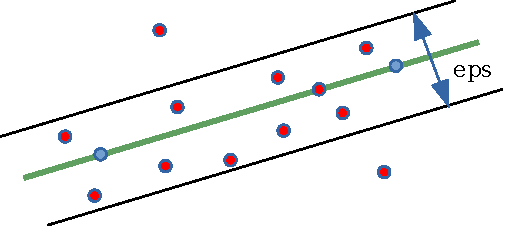
\includegraphics[width=0.6\textwidth]{bilder/ransac.pdf}
\label{ransac}
\end{center}
\end{figure}


\begin{itemize}
 \item number of iterations
 \item minimum size of the ``Consensus Set''
 \item distance threshold value (eps)
\end{itemize}

Zu beachten ist, das der \ac{RANSAC} durch die zufällige Auswahl der Datenpunkte kein deterministischer algorythmus ist.


\section{\acl{DBSCAN}}
\ac{DBSCAN} \cite{DBSCAN} ist ein deterministischer Data-Mining-Algorithmus zur Clusteranalyse. Der Algorithmus basiert auf der Dichteverbundenheit, das heißt er bindet punkte basierend auf iher Enterferung zu Clustern
\ac{DBSCAN} iterietert über alle  noch nicht beabreiteten Datenpunkte, jeder bearbeitete Datenpunkt wird als bearbeitet makiert. Für jeden dieser Pubnkte wird dann eine Berichsanfrage durchgeführt.
Ist die größe der nachbarschaft keiner als ein bestimmter Grenzwert, wird der Punkt las Rausche makiert. Andernfalls Wird ein neuer Clusrer erstellt, indem für jeden Punkt in
der nachbarschaft eine neue Bereichsanfrage durchgeführt wird, wird dieser Nicht als Rauschen klassifiziert, wird dieser zum Cluster hinzugefügt und als bearbeitet Makiert.
Dies wird solage ausgeführt, bsi alle im Cluster befeindlich punkte als Bearbeitet makiert sind, also keine Weiteren punkte in der nachbarschaft erreichbar sind.

\begin{figure}[!ht]
\begin{center}
\caption{\acs{DBSCAN} \cite{DBSCAN}}
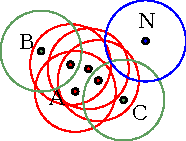
\includegraphics[width=0.6\textwidth]{bilder/dbscan.pdf}
\label{dbscan}
\end{center}
\end{figure}



Der \ac{DBSCAN} hat also zwei zu Bestimmende Parameter, welche das ergebnis beeinflussen.
\begin{itemize}
 \item maximum distance of the neighborhood points
 \item minimum number of points required to form a dense region
\end{itemize}






\section{Middleware OpenDAVINCI}
Autonome Software ist typischer weise ein verteiletes System, auf heutigen Fahrzeugen basiert dieses System auf ECUs und Bussystemen wie CAN,LIN.
Verteilete Sysoftware vereinfacht es komplexe Komponenten innheralb des Systems zu integreieren. Im bereich des Autonomen Fahrens iust der Historische aufbau von Fahrzeugen
mit ECU'S und can jedoch nicht optimal \cite{Broy2006}. Um die vielen benötigekten Komponenten zu handhaben, ist es von vorteil Komponenten auch innerhalb eines ECU's bzw einer Recheneinheit
zu entkoppeln. Für diesen Zweck gibt es beireits mehrer middelwares die unteranderm die Kommunikation innerhalb der Komponenten handhaben und abstrahieren.
m Rahmen des Copplar Projekets, wird hier die OpenDaVINCI middleware genutzt. OpenDaVINCI ist eine echtzeitfähige laufzeitumgebeung konzipiert für Autonome Fahrzeuge.
OpenDaVINCI basiert auf Hesperia \cite{Berger2010}. Die Kommunikation zwischen den Komponenten basiert in OpenDaVINCI UDP Multicast, welches eine Echtzeitfähige Kommunikation zwischen
den Komponenten  und über Recheneinheiten hinweg Ermöglicht \cite{Kurose2013}. Für die Kommunikation bietet OpenDaVINCI Time-triggered sender und Data-triggered receiver an, von welchem in folgenden der Data-triggered receiver
für die Anbindung der Software genutzt wird. Weiterhin bietet OpenDaVINCI viele weiter Funktionalitäten die das Handling von World Geodetic System 1984 (WGS84) Korridinaten an, welches für die Umwandlung
von GPS koordinaten in lokale kartesische genutzt werden kann. Dazu ist die Angabe einer referenz GPS postion nötig, welche um den Berechnugsfehler klein zu halten,
nicht zu weit entfernt sein sollte.






